\setcounter{dang}{0}
\setcounter{section}{1}
\setcounter{ex}{0}
\setcounter{vd}{0}
\setcounter{bt}{0}
\section{TẬP HỢP VÀ CÁC PHÉP TOÁN TRÊN TẬP HỢP}

\subsection{TÓM TẮT LÝ THUYẾT}

\subsubsection{Các khái niệm cơ bản về tập hợp}
\begin{enumerate}[\iconMT]
	\item \indam{Tập hợp}
	\begin{enumerate}[\faPencilSquareO]
		\item Khi muốn mô tả các đối tượng (phần tử) có chung một tính chất gì đó thì ta xây dựng khái niệm tập hợp.
		\item Cách xác định tập hợp:
		\begin{listEX}[1]
			\item [\ding{172}] Liệt kê các phần tử: viết các phần tử của tập hợp trong hai dấu móc $\left\{...\right\}$.
			\item [\ding{173}] Chỉ ra tính chất đăc trưng cho các phần tử của tập hợp.
		\end{listEX}
		\item Tập rỗng: là tập hợp không chứa phần tử nào, kí hiệu $\varnothing $.
	\end{enumerate}	
	\item \indam{Tập hợp con - Tập hợp bằng nhau}
	\begin{enumerate}[\faPencilSquareO]
		\item Tập hợp con: 
		\begin{boxdn}
			\immini{\begin{itemize}
					\item $A\subset B\Leftrightarrow (\forall x\colon x \in A\Rightarrow x\in B)$.
					\item  Các tính chất:
					\begin{listEX}[1]
						\item [\ding{172}] $A\subset A,\forall A$.
						\item [\ding{173}] $\varnothing \subset A,\forall A$.
						\item [\ding{174}] $A\subset B$, và $B\subset C$ suy ra $A\subset C$.
					\end{listEX}
			\end{itemize}}{
				\begin{tikzpicture}[smooth,font=\footnotesize,scale=1]
					\def\miena{(0,0) to[bend left=90] (2,2) to[bend left=90] (0,0)}
					\def\mienb{(0.5,0.5) to[bend left=90] (1.5,1.75) to[bend left=90] (0.5,0.5)}
					\draw[pattern=dots] \miena;
					\draw[fill=white] \mienb
					(1,-0.7) node{Biểu đồ Ven minh họa  $A \subset B$}
					(1,1.2) node{$A$}
					(0.5,0.1) node{$B$};
			\end{tikzpicture}}
		\end{boxdn}
		\item Tập hợp bằng nhau: 
		\begin{boxdn}
			\begin{itemize}
				\item[] $A=B\Leftrightarrow A\subset B$ và $B\subset A\Leftrightarrow (\forall x \colon x\in A\Leftrightarrow x\in B)$.
			\end{itemize} 
		\end{boxdn}
	\end{enumerate}
\end{enumerate}
\subsubsection {Các tập hợp số}
\begin{enumerate}[\iconMT]
	\item \indam{Các tập hợp số và mối quan hệ giữa các tập hợp số:}
	\begin{tcolorbox}[colframe=cyan,colback=white,boxrule=0.2mm]
		\begin{listEX}[3]
			\item [\ding{172}] Tập số tự nhiên $\mathbb{N}$.
			\item [\ding{173}] Tập số nguyên $\mathbb{Z}$.
			\item [\ding{174}] Tập số hữu tỉ $\mathbb{Q}$.
			\item [\ding{175}] Tập số vô tỉ $\mathbb{I}$.
			\item [\ding{176}] Tập số thực $\mathbb{R}$.
			\item [\ding{177}] Tập $\mathbb{N^*}$ ta bỏ số $0$.
		\end{listEX}
	\end{tcolorbox}
	\indamm{Mối quan hệ:}
	\begin{listEX}[2]
		\item [\ding{172}] $\mathbb{N} \subset \mathbb{Z} \subset \mathbb{Q} \subset \mathbb{R}$.
		\item [\ding{173}] $\mathbb{Q} \cup \mathbb{I}=\mathbb{R}$.
	\end{listEX}
	\item \indam{ Các tập con thường dùng của tập $\mathbb{R}$}
	\begin{listEX}[2]
		\item [\ding{172}] Khoảng $\left(a;b\right)=\left\{\left. x\in \mathbb{R}\right|a<x<b\right\}$.\\
		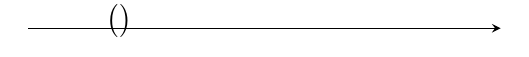
\begin{tikzpicture}[>=stealth]
			\draw[->](-1,0)->(5,0);
			\IntervalLR{-1}{1/2}
			\def\skipInterval{0.5cm}%Khoảng cách đặt nhãn
			\IntervalGRF{}{}{\big(}{a}%Gạch xọc phải qua trái
			\IntervalLR{4}{4.8}
			\def\skipInterval{0.5cm}%Khoảng cách đặt nhãn
			\IntervalGRF{\big)}{b}{}{}%Gạch xọc phải qua trái
		\end{tikzpicture}	
		\item [\ding{173}] Đoạn $\left[a;b\right]=\left\{\left. x\in \mathbb{R}\right|a\le x\le b\right\}$.\\
		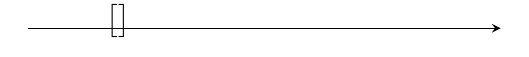
\begin{tikzpicture}[>=stealth]
			\draw[->](-1,0)->(5,0);
			\IntervalLR{-1}{1/2}
			\def\skipInterval{0.5cm}%Khoảng cách đặt nhãn
			\IntervalGRF{}{}{\big[}{a}%Gạch xọc phải qua trái
			\IntervalLR{4}{4.8}
			\def\skipInterval{0.5cm}%Khoảng cách đặt nhãn
			\IntervalGRF{\big]}{b}{}{}%Gạch xọc phải qua trái
		\end{tikzpicture}
		\item [\ding{174}] Khoảng $\left(a;+\infty \right)=\left\{\left. x\in \mathbb{R}\right|x>a\right\}$.\\
		\begin{tikzpicture}[>=stealth]
			\draw[->](-1,0)--(5,0)node[below]{$+\infty$};
			\IntervalLR{-1}{1/2}
			\def\skipInterval{0.5cm}%Khoảng cách đặt nhãn
			\IntervalGRF{}{}{\big(}{a}%Gạch xọc phải qua trái
			\IntervalLR{4}{4.8}
			\def\skipInterval{0.5cm}%Khoảng cách đặt nhãn
			%\IntervalGRF{\big]}{b}{}{}%Gạch xọc phải qua trái
		\end{tikzpicture}
		\item [\ding{175}] Nửa khoảng $\left[a;+\infty \right)=\left\{\left. x\in \mathbb{R}\right|x\ge a\right\}$.\\
		\begin{tikzpicture}[>=stealth]
			\draw[->](-1,0)->(5,0)node[below]{$+\infty$};
			\IntervalLR{-1}{1/2}
			\def\skipInterval{0.5cm}%Khoảng cách đặt nhãn
			\IntervalGRF{}{}{\big[}{a}%Gạch xọc phải qua trái
			\IntervalLR{4}{4.8}
			\def\skipInterval{0.5cm}%Khoảng cách đặt nhãn
			%\IntervalGRF{\big]}{b}{}{}%Gạch xọc phải qua trái
		\end{tikzpicture}
		\item [\ding{176}] Khoảng $\left(-\infty;b\right)=\left\{\left. x\in \mathbb{R}\right|x<b\right\}$.\\
		\begin{tikzpicture}[>=stealth]
			\draw[->](-1,0)node[below]{$-\infty$}--(5,0);
			\IntervalLR{-1}{1/2}
			\def\skipInterval{0.5cm}%Khoảng cách đặt nhãn
			%\IntervalGRF{}{}{\big[}{a}%Gạch xọc phải qua trái
			\IntervalLR{3}{4.8}
			\def\skipInterval{0.5cm}%Khoảng cách đặt nhãn
			\IntervalGRF{\big)}{b}{}{}%Gạch xọc phải qua trái
		\end{tikzpicture}
		\item [\ding{177}] Nửa khoảng $\left(-\infty;b\right]=\left\{\left. x\in \mathbb{R}\right|x\le b\right\}$.\\
		\begin{tikzpicture}[>=stealth]
			\draw[->](-1,0)node[below]{$-\infty$}->(5,0);
			\IntervalLR{-1}{1/2}
			\def\skipInterval{0.5cm}%Khoảng cách đặt nhãn
			%\IntervalGRF{}{}{\big[}{a}%Gạch xọc phải qua trái
			\IntervalLR{3}{4.8}
			\def\skipInterval{0.5cm}%Khoảng cách đặt nhãn
			\IntervalGRF{\big]}{b}{}{}%Gạch xọc phải qua trái
		\end{tikzpicture}
		\item [\ding{178}] Nửa khoảng $\left[a;b\right)=\left\{\left. x\in \mathbb{R}\right|a\le x<b\right\}$.\\
		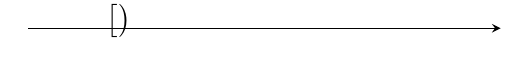
\begin{tikzpicture}[>=stealth]
			\draw[->](-1,0)->(5,0);
			\IntervalLR{-1}{1/2}
			\def\skipInterval{0.5cm}%Khoảng cách đặt nhãn
			\IntervalGRF{}{}{\big[}{a}%Gạch xọc phải qua trái
			\IntervalLR{4}{4.8}
			\def\skipInterval{0.5cm}%Khoảng cách đặt nhãn
			\IntervalGRF{\big)}{b}{}{}%Gạch xọc phải qua trái
		\end{tikzpicture}
		\item [\ding{179}] Nửa khoảng $\left(a;b\right]=\left\{\left. x\in \mathbb{R}\right|a<x\le b\right\}$.\\
		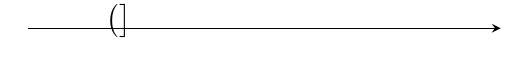
\begin{tikzpicture}[>=stealth]
			\draw[->](-1,0)->(5,0);
			\IntervalLR{-1}{1/2}
			\def\skipInterval{0.5cm}%Khoảng cách đặt nhãn
			\IntervalGRF{}{}{\big(}{a}%Gạch xọc phải qua trái
			\IntervalLR{4}{4.8}
			\def\skipInterval{0.5cm}%Khoảng cách đặt nhãn
			\IntervalGRF{\big]}{b}{}{}%Gạch xọc phải qua trái
		\end{tikzpicture}
	\end{listEX}
\end{enumerate}


\subsubsection{Các phép toán trên tập hợp}
\begin{enumerate}[\iconMT]
	\item \indam{Giao của hai tập hợp:}
	\immini{\begin{itemize}
			\item  $A\cap B= \{x|x\in A$ và $x\in B \}$.
			\item  Ghi nhớ: Lấy phần chung của 2 tập hợp.
	\end{itemize}}{
		\begin{tikzpicture}[smooth,font=\footnotesize,scale=0.8]
			\def\miena{(0,0) to[bend left=90] (2,2) to[bend left=90] (0,0)}
			\def\mienb{(1,0) to[bend left=90] (3,2) to[bend left=90] (1,0)}
			\begin{scope}
				\clip \miena;
				\draw[pattern=north east lines,pattern color=orange] \mienb;
			\end{scope}
			\draw \miena \mienb
			(1,-0.7) node{$A \cap B$}
			(0.5,1) node{$A$}
			(2.6,0.9) node{$B$};
	\end{tikzpicture}}
	\item \indam{Hợp của hai tập hợp:}
	\immini{\begin{itemize}
			\item  $A\cup B=\{x|x\in A$ hoặc $x\in B \} $.
			\item  Ghi nhớ: Gom hết phần tử của cả hai tập, các phần tử trùng nhau thì ta ghi 1 lần.
	\end{itemize}}{
		\begin{tikzpicture}[smooth,font=\footnotesize,scale=0.8]
			\draw[pattern=north east lines,pattern color=orange]
			(0,0) to[bend left=90] (2,2) to[bend left=90] (0,0)
			(1,0) to[bend left=90] (3,2) to[bend left=90] (1,0)
			(1,-0.7) node{$A \cup B$}
			(0.5,1) node{$A$}
			(2.6,0.9) node{$B$};
	\end{tikzpicture}}
	\item \indam{Hiệu của hai tập hợp:}
	\immini{\begin{itemize}
			\item  $A\backslash B= \{x|x\in A$ và $x\notin B \} $.
			\item  Ghi nhớ: Lấy phần riêng (thuộc A mà không thuộc B)
			\item Đặc biệt: Nếu $B\subset A$ thì $A\backslash B$ được kí hiệu là \fbox{$C_AB$} (gọi là phần bù của $B$ trong $A$).
	\end{itemize} }{
		\begin{tikzpicture}[smooth,font=\footnotesize,scale=0.8]
			\def\miena{(0,0) to[bend left=90] (2,2) to[bend left=90] (0,0)}
			\def\mienb{(1,0) to[bend left=90] (3,2) to[bend left=90] (1,0)}
			\fill[pattern=north east lines,pattern color=orange] \miena;
			\draw[fill=white] \mienb
			(1,-0.7) node{$A \backslash B$}
			(0.5,1) node{$A$}
			(2.6,0.9) node{$B$};
			\draw \miena ;
	\end{tikzpicture}}
\end{enumerate}

\subsection{RÈN LUYỆN KĨ NĂNG GIẢI TOÁN}
\begin{dang}{Xác định tập hợp}
\end{dang}

\begin{vd}%[0D1Y2-1]
	Cho $D=\{n \in \mathbb{N} \mid n$ là số nguyên tố, $5<n<20\}$.
	\begin{enumEX}{1}
		\item Viết tập hợp $D$ bằng cách liệt kê các phần tử. Tập hợp $D$ có bao nhiêu phần tử?
		\item Dùng kí hiệu $\in, \notin$ để viết câu trả lời cho câu hỏi sau: Trong các số $5$; $12$; $17$; $18$, số nào thuộc tập $D$, số nào không thuộc tập $D$?
	\end{enumEX}
	\loigiai{
		\begin{enumEX}{1}
			\item $D=\{7 ; 11 ; 13 ; 17 ; 19\}$. Tập hợp $D$ có $5$ phần tử.
			\item $5 \notin D$; $12 \notin D$; $17 \in D$; $18 \notin D$.
		\end{enumEX}	
	}
\end{vd}

\begin{vd}
	Viết mỗi tập hợp sau bằng cách liệt kê các phần tử.
	\begin{enumEX}{2}
		\item $A=\left\{\left. x\in \mathbb{R}\right|\left(2x-x^2\right)\left(3x-2\right)=0\right\}$.
		\item $B=\left\{\left. x\in \mathbb{Z}\right|2x^3-3x^2-5x=0\right\}$.
		\item $C=\left\{\left. x\in \mathbb{Z}\right|2x^2-75x-77=0\right\}$.
		\item $D=\left\{\left. x\in \mathbb{R}\right|(x^2-x-2)(x^2-9)=0\right\}$.
	\end{enumEX}
	\loigiai{
		\begin{enumerate}[a)]
			\item Ta giải phương trình $\left(2x-x^2\right)\left(2x^2-3x-2\right)=0\Leftrightarrow \hoac{
				& 2x-x^2=0 \\ 
				& 2x^2-3x-2=0}\Leftrightarrow \hoac{
				& x=0\vee x=2 \\ 
				& x=-\dfrac{1}{2}\vee x=2}$.\\
			Do $x\in \mathbb{R}$ nên $A=\left\{-\dfrac{1}{2};0;2\right\}$.
			\item Ta giải phương trình $2x^3-3x^2-5x=0\Leftrightarrow x\left(2x^2-3x-5\right)=0\Leftrightarrow \hoac{&x=0\\&x=-1\\&x=\dfrac{5}{3}}$.\\
			Do $x\in \mathbb{Z}$ nên $B=\left\{0;-1\right\}$.
			\item Ta giải phương trình $2x^2-75x-77=0\Leftrightarrow \hoac{&x=-1\\&x=\dfrac{77}{2}}$.\\
			Do $x\in \mathbb{Z}$ nên $C=\left\{-1\right\}$.
	\end{enumerate}}
\end{vd}

\begin{vd}
	Viết mỗi tập hợp sau bằng cách liệt kê các phần tử.
	\begin{tasks}(1)
		\task $A=\left\{\left. n\in {\mathbb{N}}^{*}\right|3<n^2<30\right\}$.
		\task $B=\left\{\left. n\in \mathbb{Z}\right|\left| n\right|<3\right\}$.
		\task $C=\left\{\left. x\right|x=3k\right.$ với $k\in \mathbb{Z}$ và $\left.-4<x<12\right\}$.
		\task $A=\left\{\left. n^2+3\right|n \in \mathbb{N} \text{ và } n<5\right\}$.
	\end{tasks}
	\loigiai{
		\begin{enumerate}[a)]
			\item Với $3<n^2<30$ và $n\in {\mathbb{N}}^{*}$ nên chọn $n=2;3;4;5$.\\
			Vậy $A=\left\{2;3;4;5\right\}$.
			\item  Vì $x<\left| 3\right|\Leftrightarrow-3<x<3$.\\
			Do $x\in \mathbb{Z}$ nên $B=\left\{-2;-1;0;1;2\right\}$.
			\item Ta có $-4<x<12\Leftrightarrow-4<3k<12\Leftrightarrow-\dfrac{4}{3}<k<4$.\\
			Do $k\in \mathbb{Z}$ nên ta chọn $k=\left\{-10;1;2;3\right\}$ suy ra $x=3k=\left\{-3;0;3;6;9\right\}$.\\
			Vậy $C=\left\{-3;0;3;6;9\right\}$.
		\end{enumerate}
	}
\end{vd}

\begin{vd}%[0D1K2-1]
	Viết mỗi tập hợp sau bằng cách nêu tính chất đặc trưng.
	\begin{enumEX}{2}
		\item $A=\{2;3;5;7\}$.
		\item $B=\{-3;-2;-1;0;1;2;3\}$.
		\item $C=\{-5;0;5;10\}$.
		\item $D=\{1;2;3;4;6;9;12;18;36\}$.
	\end{enumEX}
	\loigiai{
		\begin{enumerate}
			\item $A=\left\{x\in \mathbb{R}\big|\right. x$ nguyên tố và $\left.x<10\right\}$.
			\item $B=\left\{x\in \mathbb{Z}\big||x|\leqslant 3 \right\}$.
			\item $C=\left\{x\in \mathbb{Z}\big| x\vdots 5,-5\leqslant x\leqslant 10 \right\}$.
			\item $D=\left\{n\in \mathbb{N}\big|x \text{ là ước của } 36\right\}$.
		\end{enumerate}
	}
\end{vd}

\begin{vd}
	Trong các tập hợp sau, tập hợp nào rỗng?
	\begin{enumEX}{2}
		\item $A=\left\{\left. x\in \mathbb{R}\right|x^2-x+1=0\right\}$.
		\item $B=\left\{\left. x\in \mathbb{Q}\right|\right.x^2-4x+2\left. =0\right\}$.
		\item $C=\left\{\left. x\in \mathbb{Z}\right|\right.6x^2-7x+1\left. =0\right\}$.
		\item $D=\left\{\left. x\in \mathbb{Z}\right|\right.\left| x\right|<\left. 1\right\}$.
	\end{enumEX}
	\loigiai{
		\begin{enumEX}{1}
			\item Phương trình $x^2-x+1=0$ có $\Delta <0$ nên vô nghiệm. Do đó $A=\varnothing $.
			\item Phương trình $x^2-4x+2=0$ có hai nghiệm $x=2\pm \sqrt{2}\notin \mathbb{Q}$. Do đó $B=\varnothing $.
			\item Phương trình $6x^2-7x+1=0$ có nghiệm $x=1\in \mathbb{Z}$. Do đó $C\ne \varnothing $.
			\item Chọn $x=0\in \mathbb{Z},\left| 0\right|<1$. Do đó $D\ne \varnothing $.
		\end{enumEX}
	}
\end{vd}

\begin{dang}{Xác định tập hợp con. Hai tập hợp bằng nhau}
	Cho tập hợp $A$ gồm $n$ phần tử.
	\begin{listEX}[1]
		\item [\ding{172}] Khi liệt kê tất cả các tập con của $A$, ta liệt kê đầy đủ theo thứ tự:\\		
		\centerline{ $\varnothing$; tập $1$ phần tử; tập $2$ phần tử; tập $3$ phần tử;...; $A$.}
		\item [\ding{173}] Số tập con của $A$ là $2^n$.
		\item [\ding{174}] Số tập con gồm $k$ phần tử của $A$ là $\mathrm{C}_n^k$.
	\end{listEX}
\end{dang}
\begin{vd}
	Cho tập hợp $A=\left\{2;3;4\right\}$ và $B=\left\{2;3;4;5;6\right\}$.
	\begin{tasks}
		\task Xác định tất cả tập con có hai phần tử của $A$.
		\task Xác định tất cả tập con có ít hơn hai phần tử của $A$.
		\task Tập $A$ có tất cả bao nhiêu tập con.
		\task Xác định tất cả các tập $X$ thỏa $A \subset X \subset B$.
	\end{tasks}
\end{vd}

\begin{vd} %[0D1K2-2]%
	Cho $A=\{2;5\}, B=\{5;x\}, C=\{x;y;5\}$. Tìm các cặp số $\{x;y\}$ để $A=B=C$.
	\loigiai{
		Vì $A=B=C$ nên cả $3$ tập hợp $A$, $B$, $C$ chỉ chứa $2$ phần tử là $2$ và $5$.\\
		Do đó ta có $\left\{\begin{aligned}
			&x=2\\
			&\left[\begin{aligned}
				&y=2\\
				&y=5.\\
			\end{aligned}\right.\\
		\end{aligned}\right.$
	}
\end{vd}

\begin{dang}{Các phép toán trên tập hợp}
\end{dang}

\begin{vd}
	Cho $A$ là tập hợp các học sinh lớp 10 đang học ở trường em, $B$ là tập hợp học sinh đang học tiếng Anh ở trường em. Hãy diễn đạt bằng lời các tập hợp sau.
	
	\begin{enumEX}{4}
		\item $A\cap B$.
		\item $A\backslash B$.
		\item $A\cup B$.
		\item $B\backslash A$
	\end{enumEX}
	\loigiai{
		\begin{enumerate}
			\item $A\cap B$ là tập hợp các học sinh lớp 10 học môn Tiếng Anh của trường em.
			\item $A\backslash B$ là tập hợp các học sinh lớp 10 nhưng không học môn Tiếng Anh của trường em.
			\item $A\cup B$ là tập hợp các học sinh hoặc học lớp 10 hoặc học môn Tiếng Anh của trường em.
			\item $B\backslash A$ là tập hợp các học sinh học môn Tiếng Anh nhưng không học lớp 10 của trường em.
		\end{enumerate}
	}
\end{vd}

\begin{vd}
	Cho hai tập hợp $A=\left\{0;1;2;3;4\right\}$ và $B=\left\{2;3;4;5;6\right\}$. Tìm các tập hợp $A\cup B, A\cap B, A\backslash B, B\backslash A$.
	\loigiai{
		Ta có $A\backslash B=\left\{0;1\right\}$, $B\backslash A=\left\{5;6\right\}$, $A\cup B=\left\{0;1;2;3;4;5;6\right\}$, $A\cap B=\left\{2;3;4\right\}$.
	}
\end{vd}



\begin{vd}
	Cho $A=\left\{x\in \left. \mathbb{N}\right|\right.x\le \left. 5\right\}$, $B=\left\{x\in \left. \mathbb{N}\right|\right.x=3k-1,k\in \mathbb{N},k\le \left. 3\right\}$. Xác định tập $A, B, A\cap B, A\cup B, A\backslash B, B\backslash A$.
	\loigiai{
		Ta có $A=\left\{0;1;2;3;4;5\right\}$ và $B=\left\{2;5;8\right\}$ nên
		\begin{enumerate}
			\item $A\cap B=\left\{2;5\right\}$,
			\item $A\cup B=\left\{0;1;2;3;4;5;8\right\}$,
			\item $A\backslash B=\left\{0;1;3;4\right\}$,
			\item $B\backslash A=\left\{-1;8\right\}$.
		\end{enumerate}
	}
\end{vd}

\begin{vd}
	Cho tập hợp $E=\left\{1;2;3;4;5;6;7;8;9\right\}$ và các tập hợp con $A=\left\{1;2;3;4\right\}$, $B=\left\{2;4;6;8\right\}$. Xác định $C_EA$, $C_EB$, $C_E\left(A\cup B\right)$, $C_EA\cap C_EB$.
	\loigiai{\\
		Ta có $C_EA=E\backslash A=\left\{5;6;7;8;9\right\}$, $C_EB=E\backslash B=\left\{1;3;5;7;9\right\}$ suy ra $C_EA\cap C_EB=\left\{5;7;9\right\}$.\\
		$A\cup B=\left\{1;2;3;4;6;8\right\}$ suy ra $C_E\left(A\cup B\right)=E\backslash A\cup B=\left\{5;7;9\right\}$.
	}
\end{vd}

\begin{vd}
	Xác định hai tập $A$, $B$ biết rằng
	$A\backslash B=\left\{1;5;7;8\right\}, B\backslash A=\left\{2;10\right\}, A\cap B=\left\{3;6;9\right\}$.
	\loigiai{
		$A=\left(A\backslash B\right)\cup \left(A\cap B\right)=\left\{1;5;7;8;3;6;9\right\}$, $B=\left(B\backslash A\right)\cup \left(A\cap B\right)=\left\{2;10;3;6;9\right\}$.
	}
\end{vd}

\begin{vd}
	Cho hai tập hợp $A=\left\{1;2\right\}$ và $B=\left\{1;2;3;4\right\}$. Tìm tất cả các tập hợp $X$ sao cho $A\cup X=B$.
	\loigiai{
		Ta có $A\cup X=B\Leftrightarrow X= \{3;4\} \cup X'$ với $X' \subset \{1;2\}$.\\
		Suy ra các tập $X$ cần tìm thỏa mãn yêu cầu bài toán là $\left\{3;4\right\}, \left\{1;3;4\right\}, \left\{2;3;4\right\}, \left\{1;2;3;4\right\}$.
	}
\end{vd}

\begin{dang}{Các phép toán trên tập hợp con của tập số thực}
\end{dang}

\begin{vd}%[0D1B4]
	Xác định các tập hợp sau đây và biểu diễn chúng trên trục số.
	\begin{tasks}(3)
		\task $\left(0;3\right)\cap \left(2;4\right).$
		\task $\left[-1;4\right]\cap \left(2;5\right).$
		\task $\mathbb{R}\cap \left(-1;1\right).$
	\end{tasks}
	\loigiai{
		\begin{itemize}
			\item $\left(0;3\right)\cap \left(2;4\right)=\left(2;3\right)$.
			\begin{center}
				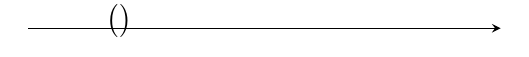
\begin{tikzpicture}[>=stealth]
			\draw[->](-1,0)->(5,0);
			\IntervalLR{-1}{1/2}
			\def\skipInterval{0.5cm}%Khoảng cách đặt nhãn
			\IntervalGRF{}{}{\big(}{2}%Gạch xọc phải qua trái
			\IntervalLR{4}{4.8}
			\def\skipInterval{0.5cm}%Khoảng cách đặt nhãn
			\IntervalGRF{\big)}{3}{}{}%Gạch xọc phải qua trái
		\end{tikzpicture}
			\end{center}
			\item $\left[-1;4\right]\cap \left(2;5\right)=\left(2;4\right]$.
			\begin{center}
				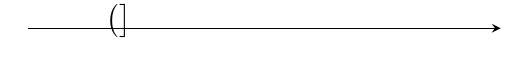
\begin{tikzpicture}[>=stealth]
			\draw[->](-1,0)->(5,0);
			\IntervalLR{-1}{1/2}
			\def\skipInterval{0.5cm}%Khoảng cách đặt nhãn
			\IntervalGRF{}{}{\big(}{2}%Gạch xọc phải qua trái
			\IntervalLR{4}{4.8}
			\def\skipInterval{0.5cm}%Khoảng cách đặt nhãn
			\IntervalGRF{\big]}{4}{}{}%Gạch xọc phải qua trái
		\end{tikzpicture}
			\end{center}
			\item $\mathbb{R}\cap \left(-1;1\right)=\left(-1;1\right)$.
			\begin{center}
				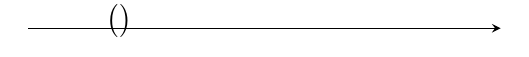
\begin{tikzpicture}[>=stealth]
			\draw[->](-1,0)->(5,0);
			\IntervalLR{-1}{1/2}
			\def\skipInterval{0.5cm}%Khoảng cách đặt nhãn
			\IntervalGRF{}{}{\big(}{-1}%Gạch xọc phải qua trái
			\IntervalLR{4}{4.8}
			\def\skipInterval{0.5cm}%Khoảng cách đặt nhãn
			\IntervalGRF{\big)}{1}{}{}%Gạch xọc phải qua trái
		\end{tikzpicture}
			\end{center}
		\end{itemize}
	}
\end{vd}

\begin{vd}%[0D1B4]
	Cho hai tập hợp $A=\lbrace x\in \mathbb{R}\vert -1\leq x \leq 3 \rbrace$, $B=\lbrace x\in \mathbb{R}\vert -2< x<2 \rbrace$. Tìm $A\cap B$.
	\loigiai{
		\begin{itemize}
			\item [] 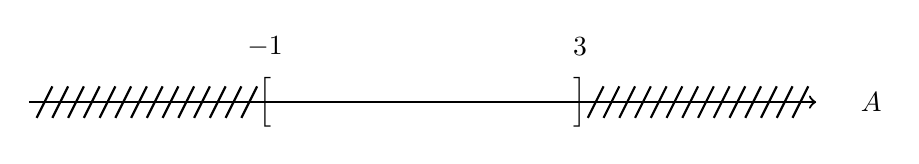
\begin{tikzpicture}[scale=1]
				\draw[->,thick](-4,0) --(6,0) node at (-1,0.7){$-1$} node at (3,0.7){$3$} node at (-1,0) {$\Big [$} node at (3,0) {$\Big ]$}node at (6.7,0){$A$};
				\foreach \b in {-3.8,-3.6,...,-1.2} {\draw[ thick](\b-0.1,-0.2)--(\b+0.1,0.2);}
				\foreach \b in {3.2,3.4,...,5.8} {\draw[ thick](\b-0.1,-0.2)--(\b+0.1,0.2);}
			\end{tikzpicture}
			\item [] 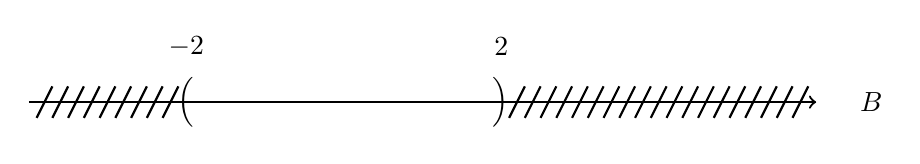
\begin{tikzpicture}[scale=1]
				\draw[->,thick](-4,0) --(6,0) node at (-2,0.7){$-2$} node at (2,0.7){$2$} node at (-2,0) {$\Big ($} node at (2,0) {$\Big )$}node at (6.7,0){$B$};
				\foreach \b in {-3.8,-3.6,...,-2.2} {\draw[ thick](\b-0.1,-0.2)--(\b+0.1,0.2);}
				\foreach \b in {2.2,2.4,...,5.8} {\draw[ thick](\b-0.1,-0.2)--(\b+0.1,0.2);}
			\end{tikzpicture}
		\end{itemize}
		$\Rightarrow A\cap B=\left[-1;2\right)$.}
\end{vd}


\begin{vd}%[0D1B4]
	Cho $A=\left[-2;4\right],B=\left(2;+\infty\right),C=(-\infty;3)$. Xác định các tập hợp sau đây và biểu diễn chúng trên trục số.
	\begin{tasks}(3)
		\task $A\cap B$;
		\task $B\cap C$;
		\task $A\cap C$;
		\task $\mathbb{R}\cap A$;
		\task $\mathbb{R}\cap B$;
		\task $A\cap B \cap C$.
	\end{tasks}
\end{vd}

\begin{vd}%[Hồ Thúy]%[0D1G4]
	Cho các tập hợp $A=\{x\in \mathbb{R}| |x+2|<2\}$, $B=\{x\in \mathbb{R}| |x+4|\geq 3\}$, $C=[-5;3)$. Tìm các tập hợp
	\begin{tasks}(3)
		\task $A \cup B$.
		\task $A \cap B \cup C$.
		\task $(A \cup B)\cap(B \cup C)$.
	\end{tasks}
\end{vd}

\begin{vd}%[0D1B4]
	Xác định các tập hợp sau đây và biểu diễn chúng trên trục số.
	\begin{tasks}(3)
		\task $\left(0;3\right)\setminus \left(2;4\right).$
		\task $\left(-4;2\right]\setminus \left[2;4\right).$
		\task $\mathbb{R}\setminus \left(-1;1\right).$
	\end{tasks}
\end{vd}

\begin{vd}%[0D1B4]
	Cho hai tập hợp $A=\lbrace x\in \mathbb{R}\vert -1\leq x \leq 3 \rbrace$, $B=\lbrace x\in \mathbb{R}\vert -2< x<2 \rbrace$. Tìm $A\setminus B, B\setminus A$.
	\loigiai{
		\begin{itemize}
			\item [] 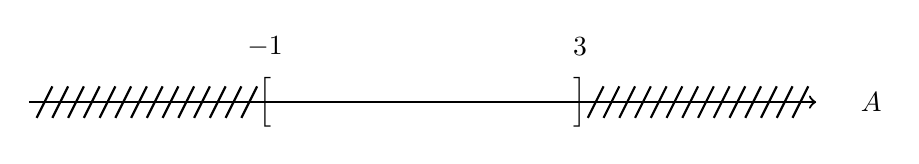
\begin{tikzpicture}[scale=1]
				\draw[->,thick](-4,0) --(6,0) node at (-1,0.7){$-1$} node at (3,0.7){$3$} node at (-1,0) {$\Big [$} node at (3,0) {$\Big ]$}node at (6.7,0){$A$};
				\foreach \b in {-3.8,-3.6,...,-1.2} {\draw[ thick](\b-0.1,-0.2)--(\b+0.1,0.2);}
				\foreach \b in {3.2,3.4,...,5.8} {\draw[ thick](\b-0.1,-0.2)--(\b+0.1,0.2);}
			\end{tikzpicture}
			\item [] 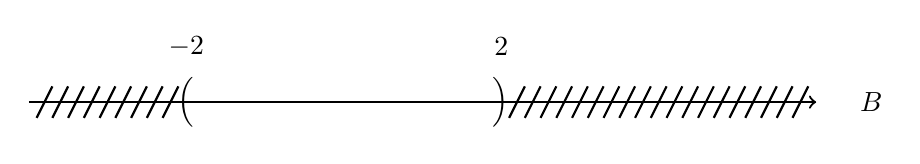
\begin{tikzpicture}[scale=1]
				\draw[->,thick](-4,0) --(6,0) node at (-2,0.7){$-2$} node at (2,0.7){$2$} node at (-2,0) {$\Big ($} node at (2,0) {$\Big )$}node at (6.7,0){$B$};
				\foreach \b in {-3.8,-3.6,...,-2.2} {\draw[ thick](\b-0.1,-0.2)--(\b+0.1,0.2);}
				\foreach \b in {2.2,2.4,...,5.8} {\draw[ thick](\b-0.1,-0.2)--(\b+0.1,0.2);}
			\end{tikzpicture}
		\end{itemize}
		$\Rightarrow A\setminus B=\left[2;3\right], B\setminus A=\left(-2;-1\right)$.}
\end{vd}
%
\begin{vd}%[0D1B4]
	Cho hai tập hợp $A=\lbrace x\in \mathbb{R}\vert 1<x\leq 4 \rbrace$, $B=\lbrace x\in \mathbb{R}\vert -3<x \rbrace$. Tìm $C_BA$.
	\loigiai{
		\begin{itemize}
			\item [] 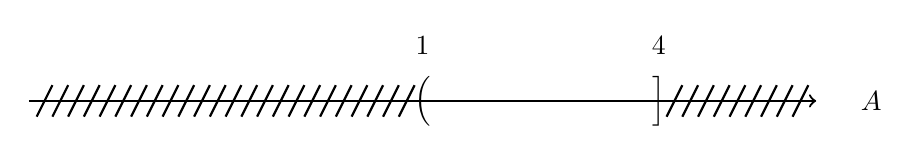
\begin{tikzpicture}[scale=1]
				\draw[->,thick](-4,0) --(6,0) node at (1,0.7){$1$} node at (4,0.7){$4$} node at (1,0) {$\Big ($} node at (4,0) {$\Big ]$}node at (6.7,0){$A$};
				\foreach \b in {-3.8,-3.6,...,0.8} {\draw[ thick](\b-0.1,-0.2)--(\b+0.1,0.2);}
				\foreach \b in {4.2,4.4,...,5.8} {\draw[ thick](\b-0.1,-0.2)--(\b+0.1,0.2);}
			\end{tikzpicture}
			\item [] \begin{tikzpicture}[scale=1]
				\draw[->,thick](-4,0) --(6,0) node at (-3,0.7){$-3$} node at (-3,0) {$\Big ($} node at (6.7,0){$B$};
				\foreach \b in {-3.8,-3.6,...,-3.2} {\draw[ thick](\b-0.1,-0.2)--(\b+0.1,0.2);}
			\end{tikzpicture}
		\end{itemize}
		$\Rightarrow C_BA=\left(-3;1\right] \cup \left(4;+\infty\right)$.
	}
\end{vd}

\begin{vd}%[0D1K4]
	Cho hai nửa khoảng $A=\left(-1;0\right],B=\left[0;1\right)$. Tìm $A\setminus B$ và $C_\mathbb{R}A$.
	\loigiai{
		\begin{itemize}
			\item [] 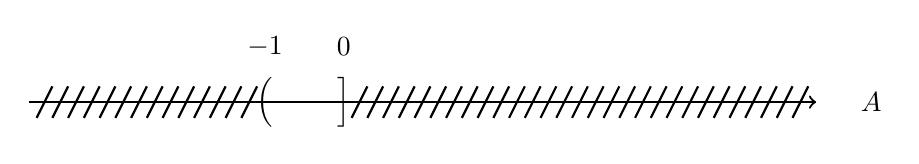
\begin{tikzpicture}[scale=1]
				\draw[->,thick](-4,0) --(6,0) node at (-1,0.7){$-1$} node at (0,0.7){$0$} node at (-1,0) {$\Big ($} node at (0,0) {$\Big ]$}node at (6.7,0){$A$};
				\foreach \b in {-3.8,-3.6,...,-1.2} {\draw[ thick](\b-0.1,-0.2)--(\b+0.1,0.2);}
				\foreach \b in {0.2,0.4,...,5.8} {\draw[ thick](\b-0.1,-0.2)--(\b+0.1,0.2);}
			\end{tikzpicture}
			\item [] 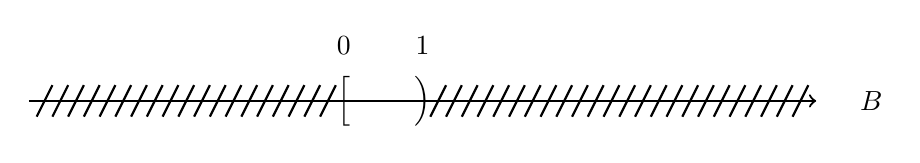
\begin{tikzpicture}[scale=1]
				\draw[->,thick](-4,0) --(6,0) node at (0,0.7){$0$} node at (1,0.7){$1$} node at (0,0) {$\Big [$} node at (1,0) {$\Big )$}node at (6.7,0){$B$};
				\foreach \b in {-3.8,-3.6,...,-0.2} {\draw[ thick](\b-0.1,-0.2)--(\b+0.1,0.2);}
				\foreach \b in {1.2,1.4,...,5.8} {\draw[ thick](\b-0.1,-0.2)--(\b+0.1,0.2);}
			\end{tikzpicture}
		\end{itemize}
		$\Rightarrow A\setminus B=\left(-1;0\right)$ và $C_\mathbb{R}A=\left(-\infty;-1\right]\cup \left(0;+\infty\right)$.\\
	}
\end{vd}

\subsection{VẬN DỤNG, THỰC TIỄN}
\begin{dang}{Các bài toán biện luận theo tham số}
\end{dang}

\begin{vd}
	Cho hai tập hợp $A=\left[-4;1\right]$, $B=\left[-3;m\right]$. Tìm $m$ để 
	\begin{enumEX}{2}
		\item $A\cap B=\left[-3;1\right]$.
		\item $A\cup B=A$
	\end{enumEX}
	\loigiai{
		Điều kiện: $m>-3$.
		\begin{enumerate}[1.]
			\item Để $A\cap B=\left[-3;1\right]$ khi và chỉ khi $m\ge 1$: thỏa mãn điều kiện.\\
			Vậy $m\ge 1$ là giá trị cần tìm.
			\item Để $A\cup B=A$ khi và chỉ khi $B\subset A$, tức là $m\le 1$.\\
			Đối chiếu điều kiện, ta được $-3<m\le 1$ là giá trị cần tìm thỏa mãn yêu cầu bài toán.
		\end{enumerate}
	}
\end{vd}

\begin{vd}
	Cho hai tập hợp $A=\left(m-1;5\right)$ và $B=\left(3;+\infty \right)$. Tìm $m$ để $A\backslash B=\varnothing $.
	\loigiai{
		Điều kiện: $m-1<5\Leftrightarrow m<6$.\\
		Để $A\backslash B=\varnothing $ khi và chỉ khi $A\subset B$, tức là $3\le m-1\Leftrightarrow m\ge 4$.\\
		Đối chiếu điều kiện, ta được $4\le m<6$.\\
		Vậy $4\le m<6$ thỏa mãn yêu cầu bài toán.
	}
\end{vd}

\begin{vd}
	Cho hai tập hợp $A=\left(-4;3\right)$ và $B=\left(m-7;m\right)$. Tìm $m$ để $B\subset A$.
	\loigiai{
		Điều kiện: $m\in \mathbb{R}$.\\
		Để $B\subset A$ khi và chỉ khi $\heva{
			& m-7\ge-4 \\ 
			& m\le 3 \\}\Leftrightarrow \heva{
			& m\ge 3 \\ 
			& m\le 3 \\}\Leftrightarrow m=3$.\\
		Vậy $m=3$ thỏa mãn yêu cầu bài toán.
	}
\end{vd}

\begin{vd}
	Cho số thực $a<0$ và hai tập hợp $A=\left(-\infty;9a\right)$, $B=\left(\dfrac{4}{a};+\infty \right)$. Tìm $a$ để $A\cap B\ne \varnothing $.
	\loigiai{
		Để hai tập hợp $A$ và $B$ giao nhau khác rỗng khi và chỉ khi $9a>\dfrac{4}{a} \Leftrightarrow 9a^2<4$ (do $a<0$)
		$\Leftrightarrow a^2<\dfrac{4}{9} \Leftrightarrow -\dfrac{2}{3}<a<0$.\\
		Vậy $-\dfrac{2}{3}<a<0$ thỏa mãn yêu cầu bài toán.
	}
\end{vd}

\begin{vd}
	Cho hai tập hợp $A=\left[-2;m+1\right]$ và $B=\left[\dfrac{1}{2};+\infty \right)$. Tìm $m$ để $A\cap B$ chỉ có đúng 1 phần tử.
	\loigiai{
		Điều kiện: $m+1>-2\Leftrightarrow m>-3$.\\
		Để $A\cap B$ chỉ có đúng 1 phần tử khi và chỉ khi $m+1=\dfrac{1}{2}\Leftrightarrow m=-\dfrac{1}{2}$ (thỏa mãn điều kiện).\\
		Vậy $m=-\dfrac{1}{2}$.
	}
\end{vd}
\begin{dang}{Ứng dụng thực tế các phép toán tập hợp}
\end{dang}

\begin{vd}%[0D1B3-3]
	Trong kì thi học sinh giỏi cấp trường, lớp 10C1 có $45$ học sinh trong đó có  $17$ bạn đạt học sinh giỏi Văn, $25$ bạn đạt học sinh giỏi Toán và $13$ bạn học sinh không đạt học sinh giỏi. Tìm số học sinh giỏi cả Văn và Toán của lớp 10C1.
	\loigiai{
		\immini{
			\textbf{Cách 1:}\\
			Số học sinh giỏi ít nhất một trong hai môn Văn hoặc Toán là $45-13=32$.\\
			Số học sinh giỏi Văn nhưng không giỏi Toán là $32-25=7$ (bạn).\\
			Số học sinh giỏi cả Văn và Toán là $17-7=10$ (bạn).\\
			\textbf{Cách 2:} \textit(Sử dụng công thức tính nhanh - Trắc nghiệm)\\
			\begin{itemize}			
				\item Gọi $A$, $B$ theo thứ tự là tập hợp các học sinh giỏi Văn và giỏi Toán của lớp. 
				Theo đề ta có $n(A)=17$, $n(B)=25$, $n(A \cup B)= 45-13=32$.
				\item Số học sinh giỏi cả Văn và Toán là $$n(A \cap B )=n(A) + n(B) - n(A \cup B)=25+17-32=10.$$
			\end{itemize}
		}
		{	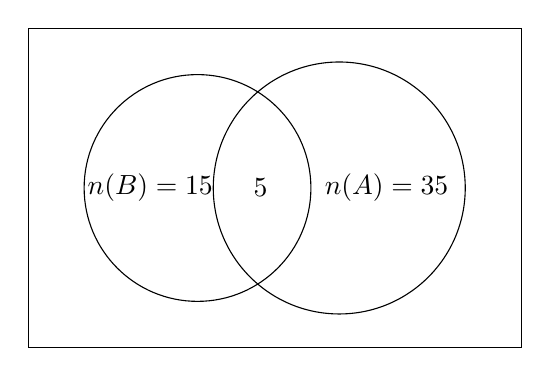
\begin{tikzpicture}[scale=.8]
				\def\radius{2cm}	
				\coordinate (ceni);
				\coordinate[xshift=.9*\radius] (cenii);
				
				\draw (ceni) circle (.9*\radius);
				\draw (cenii) circle (\radius);
				\draw  ([xshift=-25pt,yshift=15pt]current bounding box.north west) 
				rectangle ([xshift=25pt,yshift=-15]current bounding box.south east);
				
				\node[xshift=-.3*\radius] at (ceni) {$n(B)=15$};
				\node[xshift=.3*\radius] at (cenii) {$n(A)=35$};
				\node[xshift=.4*\radius] at (ceni) {$5$};
	\end{tikzpicture}}}
\end{vd}
\begin{vd}%[0D1B3-3]
	Một lớp học có $ 50 $ học sinh trong đó có $ 30 $ em biết chơi bóng chuyền, $25$ em biết chơi bóng đá, $ 10 $ em biết chơi cả bóng đá và bóng chuyền. Hỏi có bao nhiêu em không biết chơi môn nào trong hai môn ở trên?
	\loigiai{
		\textbf{Cách 1:}\\
		Số học sinh chỉ biết chơi bóng chuyền là $30-10=20$ (hs).\\
		Số học sinh biết chơi bóng đá hoặc bóng chuyền là $20+25=45$ (hs).\\
		Số học sinh không biết chơi môn nào là $50-45=5$ (hs).\\
		\textbf{Cách 2:} \textit(Sử dụng công thức tính nhanh - Trắc nghiệm)\\
		Gọi tập $A$ là tập hợp các học sinh biết chơi bóng chuyền, $B$ là tập hợp các học sinh biết chơi bóng đá.\\
		Khi đó số học sinh biết chơi ít nhất một trong hai môn bóng chuyền hoặc bóng đá là 
		$$n(A \cup B)=n(A)+n(B)-n(A \cap B)=30+25-10=45.$$
		Vậy số học sinh không biết chơi môn nào là $50-45=5$. 		
	}	
\end{vd}

\begin{vd}%[0D1B3-3]
	Lớp $10A$ có $15$ bạn thích môn Văn, $20$ bạn thích môn Toán. Trong số các bạn thích văn hoặc toán có $8$ bạn thích cả $2$ môn. Trong lớp vẫn còn $10$ bạn không thích môn nào trong $2$ môn Văn và Toán. Hỏi lớp $10A$ có bao nhiêu học sinh?
	\loigiai{Ta sử dụng sơ đồ Ven.		
		\begin{center}
			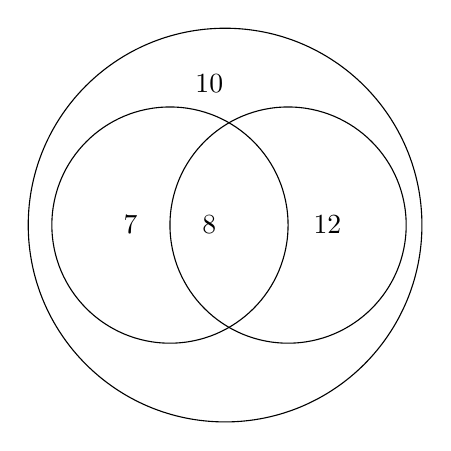
\begin{tikzpicture}
				\draw[] (0.7,0) circle ( 2.5cm);
				\draw[] (0,0) circle ( 1.5cm);
				\draw (1.5,0) circle ( 1.5 cm);
				\draw (-0.5,0) node {$7$};
				\draw (2,0) node {$12$};
				\draw (0.5,0) node {$8$};
				\draw (0.5,1.8) node {$10$};
			\end{tikzpicture}
		\end{center}
		\begin{itemize}
			\item Hình tròn lớn ngoài cùng thể hiện số học sinh cả lớp.\\
			Như vậy, ta có:\\
			\item	Số bạn chỉ thích Văn là $ 15-8=7$(bạn).\\
			\item	Số bạn chỉ thích Toán là $20-8=12$(bạn).\\
			\item	Số học sinh cả lớp là tổng các phần không giao nhau: $7+8+12+10=37$.
		\end{itemize}
	}
\end{vd}

\begin{vd}%[0D1K3-3]
	Kết quả thi học kì một của một trường THPT có $48$ thí sinh giỏi môn Toán, $37$ thí sinh giỏi môn Vật Lí,$42$ thí sinh giỏi môn Văn. Biết rằng có $75$ thí sinh giỏi môn Toán hoặc môn Vật lí, $76$ thí sinh giỏi  môn Toán hoặc môn Văn, $66$ thí sinh giỏi môn Vật lí hoặc môn Văn và có $4$ thí sinh giỏi cả ba môn. Hỏi 
	\begin{enumerate}
		\item có bao nhiêu học sinh chỉ giỏi 1 môn.
		\item có bao nhiêu học sinh chỉ giỏi 2 môn.
		\item có bao nhiêu học sinh giỏi ít nhất 1 môn.
	\end{enumerate}
	\loigiai{
		\immini{		
			Gọi $A$, $B$, $C$ theo thứ tự là tập hợp các học sinh giỏi Toán, giỏi Lí và giỏi Văn. Theo đề ta có
			\begin{itemize}
				\item Số học sinh giỏi Toán và Lí là $n(A \cap B)=n(A)+n(B)-n(A \cup B)=48+37-75=10.$
				\item Số học sinh giỏi Toán và Văn là $n(A \cap C)=n(A)+n(C)-n(A\cup C)=48+42 - 76 = 14 .$
				\item Số học sinh giỏi Lí và Văn là $n(B \cap C)=n(B)+n(C)-n(B\cup C)= 42+37-66=13 .$
				\item Số học sinh chỉ giỏi Toán và Lí là $10-4=6$.
				\item Số học sinh chỉ giỏi Toán và Văn là $14-4=10$.
				\item Số học sinh chỉ giỏi Lí và Văn là $13-4=9$.	
				\item Số học sinh chỉ giỏi môn Toán $48-10-6-4=28$.	
				\item Số học sinh chỉ giỏi môn Lí $37-6-4-9=18 $.	
				\item Số học sinh chỉ giỏi môn Văn $42-10-9-4=19 $.
			\end{itemize}
		}{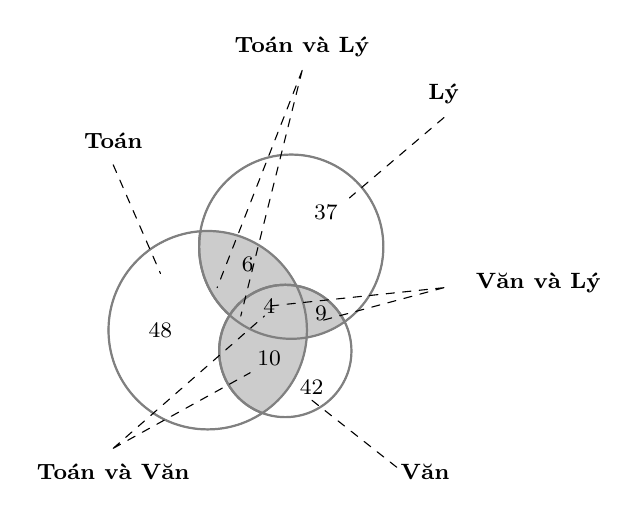
\begin{tikzpicture}[scale=0.6,>=stealth, font=\footnotesize, line join=round, line cap=round]	
				\def\firstcircle{(0,0) circle (2.1cm)}
				\def\secondcircle{(45:2.5cm) circle (1.95cm)}
				\def\thirdcircle{(-15:1.7cm) circle (1.4cm)}
				\colorlet{circle edge}{black!50}
				\colorlet{circle area}{black!20}
				\tikzset{filled/.style={fill=circle area, draw=circle edge, thick},
					outline/.style={draw=circle edge, thick}}
				\draw \firstcircle;
				\draw \secondcircle;
				\draw \thirdcircle;
				\begin{scope}
					\clip \firstcircle;
					\fill[filled] \secondcircle;
				\end{scope}
				\begin{scope}
					\clip \firstcircle;
					\fill[filled] \thirdcircle;
				\end{scope}
				\begin{scope}
					\clip \secondcircle;
					\fill[filled] \thirdcircle;
				\end{scope}  
				\node at (-1,0){48};  
				\node at (2.2,-1.2){42};     
				\node at (2.5,2.5){37}; 
				%
				\node at (0.85,1.4){6}; 
				\node at (1.3,0.5){4}; 
				\node at (1.3,-0.6){10}; 
				\node at (2.4,0.35){9}; 
				\draw[outline] \firstcircle
				\secondcircle  \thirdcircle;    
				\node at (-2,4) {\textbf{Toán}};
				\node at (2,6) {\textbf{Toán và Lý}};
				\node at (5,5) {\textbf{Lý}};
				\node at (7,1) {\textbf{Văn và Lý}};   
				\node at (4.6,-3) {\textbf{Văn}};
				\node at (-2,-3) {\textbf{Toán và Văn}};
				\draw[dashed] (-2,3.5) -- (-1,1.2) 
				(2,5.5) -- (0.7,0.3) 
				(2,5.5) -- (0.2,0.9)
				(5,4.5) -- (3,2.8)
				(5,0.9) -- (1.2,0.5)
				(5,0.9) -- (2.4,0.2)
				(4,-2.9) -- (2.1,-1.4)
				(-2,-2.5) -- (1.2,0.3)
				(-2,-2.5) -- (0.9,-0.9)	;
		\end{tikzpicture}}
		\begin{enumerate}	
			\item Số học sinh chỉ giỏi đúng 1 môn là $28+18+19=65$. 
			\item Số học sinh chỉ giỏi đúng 2 môn là $10+6+9=25$. 
			\item Số học sinh giỏi ít nhất một môn là $65+25+4=94$.
		\end{enumerate}
		\textbf{Cách 2:} Đặt $x,y,z$ lần lượt là số học sinh chỉ giỏi Toán, chỉ giỏi Lí, chỉ giỏi Văn; $a,b,c$ là số học sinh chỉ giỏi Toán và Lí, chỉ giỏi Toán và Văn, chỉ giỏi Lí và Văn.\\
		Khi đó ta có hệ phương trình
		$$\heva{& x+a+b+4=48\\
			&y+a+c+4=37\\
			&z+b+c+4=42\\
			&x+y+a+b+c+4=75\\
			&x+z+a+b+c+4=76\\
			&y+z+a+b+c+4=66} 
			\Rightarrow \heva{& x+y+z+2(a+b+c)+12= 127\\ & 2(x+y+z)+3(a+b+c)+12= 217}
			\Rightarrow \heva{& x+y+z= 65\\ & a+b+c= 25}.$$
		Từ đó ta có
		\begin{itemize}
			\item Số học sinh chỉ giỏi đúng một môn là $x+y+z=65$.
			\item Số học sinh chỉ giỏi đúng hai môn là $a+b+c=25$.
			\item Số học sinh giỏi ít nhất một môn là $65+25+4=94$.
		\end{itemize}
		}
\end{vd}

\subsection{BÀI TẬP TỰ LUYỆN}
\begin{bt}%[0D1B2-1]
	Liệt kê các phần tử của các tập hợp sau:
	\begin{enumerate}
		\item $A=\left\lbrace n\in \mathbb{N} \mid n<5\right\rbrace$.
		\item $B$ là tập hợp các số tự nhiên lớn hơn $0$ và nhỏ hơn $5$.
		\item $C=\left\lbrace x\in \mathbb{R}\mid (x-1)(x+2)=0\right\rbrace$.
	\end{enumerate}
	\loigiai{
		\begin{enumerate}
			\item $A=\left\lbrace 0;1;2;3;4\right\rbrace$.
			\item $B=\left\lbrace 1;2;3;4\right\rbrace$.
			\item Ta có $(x-1)(x+2)=0 \Leftrightarrow \hoac{&x=1\\&x=-2.}$\\
			Mà $x\in \mathbb{R}$ nên
			$C=\left\lbrace -2;1\right\rbrace$.
		\end{enumerate}
	}
\end{bt}
\begin{bt}%[0D1B2-1]
	Viết các tập hợp sau bằng phương pháp liệt kê
	\begin{tasks}(2)
		\task $A=\left\lbrace  x\in \mathbb{Q}\mid (x^2-2x+1)(x^2-5)\right\rbrace=0$.
		\task $B=\left\lbrace x \in \mathbb{N}\mid 5<x^2<40\right\rbrace$.
		\task $C=\left\lbrace x\in \mathbb{Z}\mid x^2<9\right\rbrace$.
		\task $D=\left\lbrace x\in \mathbb{R}\mid \left|2x+1\right|=5\right\rbrace$.
	\end{tasks}
	\loigiai{
		\begin{enumerate}[a)]
			\item Ta có $x\in A\Leftrightarrow\hoac{&x^2-2x+1=0\\&x^2-5=0}\Leftrightarrow\hoac{&x=1\in\mathbb{Q}\\&x=\pm\sqrt{5}\not\in \mathbb{Q}.}$\\
			Vậy $A=\left\lbrace 1\right\rbrace$.
			\item $B=\left\lbrace 3;4;5;6\right\rbrace$.
			\item $C=\left\lbrace -2;-1;0;1;2\right\rbrace$.
			\item Ta có $\left|2x+1\right|=5\Leftrightarrow \hoac{&x=2\\&x=-3.}$\\
			Vậy $C=\left\lbrace 2;-3\right\rbrace$.
		\end{enumerate}
	}
\end{bt}
\begin{bt}
	Cho các tập hợp sau
	\begin{itemize}
		\item [] $A=\left\{\left. x\in \mathbb{Z}\right|-1\le x<6\right\}$;
		\item [] $B=\left\{\left. x\in \mathbb{Q}\right|\left(1-3x\right)\left({x}^4-3x^2+2\right)=0\right\}$;
		\item [] $C=\left\{0;1;2;3;4;5;6\right\}$.
	\end{itemize}
	\begin{tasks}
		\task Viết các tập hợp $A, B$ dưới dạng liệt kê các phần tử.
		\task Tìm $A\cap B,A\cup B,A\backslash B,{C}_{B\cup A}\left(A\cap B\right)$.
		\task Chứng minh rằng $A\cap (B\cup C)=A.$
	\end{tasks}
	\loigiai{
		\begin{enumerate}
			\item Ta có $A=\left\{-1; 0; 1; 2; 3; 4; 5\right\}$, $B=\left\{-1;\dfrac{1}{3};1\right\}$.
			\item Suy ra $A\cap B=\left\{-1;1\right\}$, $A\cup B=\left\{-1;0;\dfrac{1}{3};1;2;3;4;5\right\}$, $A\backslash B=\left\{0;2;3;4;5\right\}$ và ${C}_{B\cup A}\left(A\cap B\right)=\left\{0;\dfrac{1}{3};2;3;4;5\right\}$.
			\item Ta có $B\cup C=\left\{-1;0;1/3;1;2;3;4;5;6\right\}$ suy ra $A\cap \left(B\cup C\right)=\left\{-1;0;1;2;3;4;5\right\}=A$.
		\end{enumerate}
	}
\end{bt}

\begin{bt}
	Cho hai tập $A$, $B$ khác $\varnothing $, $A\cup B$ có $6$ phần tử, số phần tử của $A\cap B$ bằng nửa số phần tử của $B$. Hỏi $A$, $B$ có thể có bao nhiêu phần tử?
	\loigiai{
		Gọi $x$ là số phần tử của $A$ và $y$ là số phần tử của $B$ với $x,y\in {\mathbb{Z}}^{+}$. Ta có: 
		\begin{itemize}
			\item $n(A \cap B)=\dfrac{1}{2}y \Rightarrow y $ là số chẵn.
			\item $n(A\cup B)=n(A)+n(B)-n(A \cap B) \Leftrightarrow 6=x+y-\dfrac{1}{2}y \Leftrightarrow x+\dfrac{1}{2}y=6$.
			\item Mặt khác $n(A) \geq n(A \cap B)$, suy ra $ x \geq \dfrac{1}{2}y$.
		\end{itemize}
		Xét 
		$$x+\dfrac{1}{2}y \geq \dfrac{1}{2}y+\dfrac{1}{2}y \Leftrightarrow 6 \geq y; \text{ mà } y \text{ chẵn nên } y \in \{2;4;6\}. $$
		Từ đây ta có ba khả năng sau:
		\begin{itemize}
			\item [$\bullet$] Nếu $y=2$ thì $x=5$ hay tập $A$ có 5 phần tử, tập $B$ có 2 phần tử và số phần tử chung là 1 phần tử.
			\item [$\bullet$] Nếu $y=4$ thì $x=4$ hay tập $A$ có 4 phần tử, tập $B$ có 4 phần tử và số phần tử chung là 2 phần tử.
			\item [$\bullet$] Nếu $y=6$ thì $x=3$ hay tập $A$ có 3 phần tử, tập $B$ có 6 phần tử và số phần tử chung là 3 phần tử.
		\end{itemize}
	}
\end{bt}

\begin{bt}
	Cho các tập hợp
	\begin{itemize}
		\item [] $A=\left\{\left. x\in \mathbb{R}\right|\left({x}^2+7x+6\right)\left(x^2-4\right)=0\right\}$
		\item [] $B=\left\{\left. x\in \mathbb{N}\right|2x\le 8\right\}$
		\item [] $C=\left\{\left. 2x+1\right|x\in \mathbb{Z}\right.$ và $\left.-2\le x\le 4\right\}$.
	\end{itemize}
	\begin{tasks}
		\task Hãy viết lại các tập hợp $A, B, C$ dưới dạng liệt kê các phần tử.
		\task Tìm $A\cup B$, $A\cap B$, $B\backslash C$, ${C}_{A\cup B}\left(B\backslash C\right)$.
		\task Tìm $\left(A\cup C\right)\backslash B$.
	\end{tasks}
	
	\loigiai{
		\begin{enumerate}
			\item Phương trình $\left({x}^2+7x+6\right)\left(x^2-4\right)=0\Leftrightarrow \hoac{
				& x^2+7x+6=0 \\ 
				& x^2-4=0 \\}\Leftrightarrow \hoac{
				& x=-1\vee x=-6 \\ 
				& x=-2\vee x=2 \\}$.\\
			Vậy $A=\left\{-6;-2;-1;2\right\}$.\\
			Ta có $\heva{
				& x\in \mathbb{N} \\ 
				& 2x\le 8 \\}\Leftrightarrow \heva{
				& x\in \mathbb{N} \\ 
				& x\le 4 \\}\Leftrightarrow x\in \left\{0,1,2,3,4\right\}$. Vậy $B=\left\{0;1;2;3;4\right\}$.\\
			Ta có $\heva{
				& x\in \mathbb{Z} \\ 
				&-2\le x\le 4 \\}\Leftrightarrow x\in \left\{-2,-1,0,1,2,3,4\right\}$. Vậy $C=\left\{-3;-1;1;3;5;7;9\right\}$.
			\item Suy ra $A\cup B=\left\{-6;-2;-1;0;1;2;3;4\right\}$, $A\cap B=\left\{2\right\}$, $B\backslash C=\left\{0;2;4\right\}$, 
			${C}_{A\cup B}\left(B\backslash C\right)=\left(A\cup B\right)\backslash \left(B\backslash C\right)=\left\{-6;-2;-1;1;3\right\}$.
			\item Ta có $A\cup C=\left\{-6;-3;-2;-1;1;2;3;5;7;9\right\}$. Suy ra $(A\cup C)\backslash B=\left\{-6;-3;-2;-1;5;7;9\right\}$.
		\end{enumerate}
	}
\end{bt}

\begin{bt}%[Nguyễn Đắc Giáp]%[0D1B4-2]
	Cho đoạn $A=[-5;1]$ và khoảng $B=(-3;2)$. Xác định $A\cup B$, $A\cap B$, $A\setminus B$, $C_{\mathbb{R}}B$.
	\loigiai{
		Ta có
		\begin{itemize}
			\item $A\cup B=[-5;2)$.
			\item $A\cap B=(-3;1]$.
			\item $A\setminus B=[-5;-3]$.
			\item $C_{\mathbb{R}}B=\mathbb{R}\setminus B=(-\infty;-3]\cup [2;+\infty)$.
		\end{itemize} 
	}
\end{bt}

\begin{bt}%[Nguyễn Đắc Giáp]%[0D1B4-1]
	Cho các tập hợp $A=\left\{x\in \mathbb{R}\big|x^2\leqslant 4\right\}$, $B=\left\{x\in \mathbb{R}\big|x<1\right\}$. Viết các tập hợp sau đây $A\cup B$, $A\cap B$, $A\setminus B$, $ C_{\mathbb{R}}B$ dưới dạng các khoảng, nửa khoảng, đoạn.
	\loigiai{
		Ta có $A=[-2;2]$ và $B=(-\infty;1)$, suy ra
		\begin{itemize}
			\item $A\cup B=[-2;2]\cup (-\infty;1)=(-\infty;2]$.
			\item $A\cap B=[-2;2]\cap (-\infty;1)=[-2;1)$.
			\item $A\setminus B=[-2;2]\setminus (-\infty;1)=[1;2]$.
			\item $C_{\mathbb{R}}B=[1;+\infty)$.
		\end{itemize}
	}
\end{bt}

\begin{bt}%[0D1B2-1]
	Viết các tập hợp sau bằng phương pháp nêu ra tính đặc trưng.
	\begin{enumEX}{2}
		\item $ A=\{1,2,3,4,5,6,7,8,9 \} $.%\dapso{$ A=\{x \in \mathbb{N^*} | x<10\} $}
		\item $ D=\{1,2,4,8,16,32,64,128,256,512\} $.%\dapso{$D=\{2^n | n \in \mathbb{N}, n \le 9 \} $}
		\item Tập hợp các số chẵn.%\dapso{$ E=\{2n | n \in \mathbb{Z}\} $}
		\item Tập hợp các số lẻ.%\dapso{$ F=\{2n+1 | n \in \mathbb{Z}\} $}
	\end{enumEX}
	\loigiai{
		\begin{enumEX}{2}
			\item $ A=\{x \in \mathbb{N^*} | x<10\} $.
			\item $ D=\{2^n | n \in \mathbb{N}, n \le 9 \} $.
			\item $ E=\{2n | n \in \mathbb{Z}\} $.
			\item  $ F=\{2n+1 | n \in \mathbb{Z}\} $.
		\end{enumEX}
	}
\end{bt}

\begin{bt}%[0D1K2-1]
	Viết mỗi tập hợp sau đây theo cách nêu tính chất đặc trưng.
	\begin{tasks}(1)
		\task Tập hợp các điểm $M$ trên mặt phẳng $(P)$, thuộc đường tròn tâm $O$ và đường kính $2R$.
		\task Tập hợp các điểm $M$ trên mặt phẳng $(P)$, thuộc hình tròn tâm $O$.
	\end{tasks}
	\loigiai{
		\begin{enumerate}[a)]
			\item $A=\left\{M\in (P)\big| OM=R \text{ với } O \text{ cố định cho trước}\right\}$.
			\item $B=\left\{M\in (P)\big| OM\leqslant R\text{ với } O \text{ cố định cho trước}\right\}$.
		\end{enumerate}
	}
\end{bt}

\begin{bt}
	Cho các tập hợp $A=\{1 ; 2 ; 3 ; 4 ; 5\}$ và $B=\{1 ; 3 ; 5 ; 7 ; 9\}$. Hãy tìm tập hợp $M$ có nhiều phần tử nhất thoả mãn $M \subset A$ và $M \subset B$.
	\loigiai{
		Vì $M \subset A$ và $M \subset B$ nên $M \subset A \cap B$.\\
		Do đó $M=\{1;3;5\}$ là tập hợp có nhiều phần tử nhất.
	}
\end{bt}

\begin{bt} %[0D1B2-2]%
	Hãy xét quan hệ bao hàm các tập hợp sau:
	\begin{itemize}
		\item [] $A$ là tập hợp các tam giác.
		\item [] $B$ là tập hợp các tam giác đều.
		\item [] $C$ là tập hợp các tam giác cân.
	\end{itemize}
	\loigiai{
		Dễ dàng nhận thấy  $B \subset C \subset A$}
\end{bt}

\begin{bt}%[0D1B2-2]
	Cho tập $X=\{1;2;3;4;5;6;7\}$.
	\begin{listEX}[1]
		\item Hãy tìm tất cả các tập con của $X$ có chứa các phần tử $1$, $3$, $5$, $7$.
		\item Có bao nhiêu tập con của $X$ chứa đúng $2$ phần tử ?
	\end{listEX}
	\loigiai{
		\begin{enumerate}
			\item[a)] Các tập con của $X$ chứa có các phần tử $1$, $3$, $5$, $7$ được thành lập bằng cách thêm vào tập $\left\{1;3  ;5;7\right\}$ các phần tử còn lại của tập $X$. Do đó tất cả các tập con của $X$ có chứa các phần tử $1$, $3$, $5$, $7$ là: $\left\{1;3  ;5;7\right\}$, $\left\{1;3  ;5;7;2\right\}$, $\left\{1;3  ;5;7;4\right\}$, $\left\{1;3  ;5;7;6\right\}$, $\left\{1;3  ;5;7;2;4\right\}$, $\left\{1;3  ;5;7;2;6\right\}$, $\left\{1;3  ;5;7;4;6\right\}$ và $X$.
			\item[b)]  Giả sử tập cần tìm là $\{a;b\}$ với $a, b\in X$ $a\ne b$.
			\begin{itemize}
				\item Vì $X$ có $7$ phần tử nên có 7 cách chọn phần tử $a$.
				\item Sau khi chọn $a$ thì $X$ còn 6 phần tử, do đó với mỗi cách chọn $a$, ta có 6 cách chọn phần tử $b$ như vậy có $7.6=42$ cặp $(a;b)$ theo cách chọn này.
			\end{itemize}
			Nhưng với cách chọn trên thì với hai phần tử bất kì $a, b$ ta đã chọn lặp lại hai lần đó là hai cặp $(a;b)$ và $(b;a)$.\\
			Do đó, có $\dfrac{42}{2}=21$ tập con của $X$ chứa đúng hai phần tử.
		\end{enumerate}
	}
\end{bt}

\begin{bt}
	Cho hai tập hợp $A=\{2 k+1 \mid k \in \mathbb{Z}\}$ và $B=\{6 l+3 \mid l \in \mathbb{Z}\}$. Chứng minh rằng $B \subset A$.
	\loigiai{
		Lấy phần tử $x$ tuỳ ý của $B$, ta có $x=6 l+3, l \in \mathbb{Z}$.\\
		Ta viết $x=2 \cdot 3 l+2+1=2(3 l+1)+1=2 k+1$ với $k=3 l+1 \in \mathbb{Z}$. Suy ra $x \in A$.\\
		Vậy, với mọi $x \in B$ ta đều có $x \in A$. Do đó, $B \subset A$.}
\end{bt}

\begin{bt}
	Cho hai tập hợp $A=\{1 ; 2 ; a\}$ và $B=\left\{1 ; a^{2}\right\}$. Tìm tất cả các giá trị của $a$ sao cho $B \subset A$.
	\loigiai{
		Ta có $B \subset A$ nếu $a^{2}=1$ hoặc $a^{2}=2$ hoặc $a^{2}=a$.\\
		Từ đó tìm được các giá trị của $a$ là: $-\sqrt{2} ;-1 ; 0 ; 1 ; \sqrt{2}$.}
\end{bt}

\begin{bt}%[Trịnh Văn Xuân, latex-k10]%[0D1B4-1]
	Cho hai tập hợp $A=[0;3]$ và $B=[a;a+2]$. Tìm $a$ để $B\subset A$.
	\loigiai{
		Điều kiện: $a\in \mathbb{R}$.\\
		Để $B\subset A$ khi và chỉ khi $\left\{\begin{aligned}
			&a\geqslant 0\\
			&a+2\leqslant 3
		\end{aligned}\right. \Leftrightarrow \left\{\begin{aligned}
			&a\geqslant 0\\
			&a\leqslant 1
		\end{aligned}\right. \Leftrightarrow 0\leqslant a\leqslant 1$.\\
		Vậy $0\leqslant a\leqslant 1$ thỏa mãn yêu cầu bài toán.
		
	}
\end{bt}

\begin{bt}
	Cho các tập hợp $A=\{x \in \mathbb{R} \mid-3 \leq x \leq 5\} ; B=[m-1 ; 6)$. Tìm $m$ để $A \cap B \neq \varnothing$.
	\loigiai{
		Ta có $A=[-3;5]$ và $B=[m-1;6)$.\\
		$A \cap B \neq \varnothing$ khi và chỉ khi $m-1 \le 5 \Leftrightarrow m \le 6$.
	}
\end{bt}

\begin{bt}
	Cho $A=(-\infty ; m+1) ; B=[3 ;+\infty)$, với $m$ lả tham số thực. Tìm $m$ để
	\begin{enumerate}
		\item $A \cup B=\mathbb{R}$
		\item $A \cap B$ chứa đúng 5 số nguyên.
	\end{enumerate}
	\loigiai{
		\begin{enumerate}
			\item $A \cup B=\mathbb{R}$ khi và chỉ khi $m+1 \ge 3 \Leftrightarrow m \ge 2$.
			\item Ta có $A \cap B \ne \varnothing$ khi và chỉ khi $m+1 > 3 \Leftrightarrow m > 2$.\\
			Khi đó $A \cap B=(-\infty ; m+1) \cap [3 ;+\infty)=\left[3 ; m+1\right)$.\\
			$A \cap B$ chứa đúng $5$ số nguyên khi và chỉ khi $3,4,5,6,7 \in [3;m+1)$ và $n \notin [3;m+1), \forall n \ge 8 $ $\Leftrightarrow 7< m+1 \le 8 \Leftrightarrow 6<m \le 7$.\\
			Vậy $m=5$ là giá trị duy nhất th
		\end{enumerate}
	}
\end{bt}

\begin{bt}
	Cho $A=[m ; m+2]$ và $B=[n ; n+1]$ với $m, n$ là các tham số thực. Tìm điều kiện của các số $m$ và $n$ để tập hợp $A \cap B$ chứa đúng một phần tử.
	\loigiai{
		Để $A \cap B$ chứa đúng một phần tử thì ta cần có $m=n+1$ hoặc $n=m+2$.
	}
\end{bt}

\begin{bt}
	Cho $U=\left\{3 ; 5 ; a^{2}\right\} ; A=\{3 ; a+4\}$, với $a$ là tham số thực. Tìm các giá trị của $a$ sao cho $C_{U} A=\{1\}$.
	\loigiai{
		Ta có $C_{U} A=\{1\} \Leftrightarrow \{5;a^2\} \setminus \{a+4\}=\{1\}$.\\
		Do đó $a+4=5$ và $a^2=1$. Do vậy $a=1$.
	}
\end{bt}

\begin{bt}
	Cho các tập hợp $A=\{x \in \mathbb{Z} \mid-2 \leq x<3\}, B=\left\{0 ; m^{2}+1 ; m^{2}+2\right\}$. Có bao nhiêu giá trị của tham số $m$ để $B \subset A$.
	\loigiai{
		Ta có $A=\{-2;-1;0;1;2\}$.\\
		Để $B \subset A$ thì $0 \in A$ và $m^2+1, m^2+2 \in A$.\\
		Từ đó suy ra $m^2+1=1$ và $m^2+2=2$ (vì $m^2 \ge 0$).\\
		Do đó $m=0$ là giá trị cần tìm.
\end{bt}

\begin{bt}
	Cho tập $A=\left\{x \in \mathbb{Z} \mid(x+2)\left(5 x^{2}-6 x+1\right)=0\right\}$. Với $m$ là số thực, xét tập $B=\left\{x \in \mathbb{R} \mid x^{2}-(2 m+1) x+2 m=0\right\}$. Tìm $m$ để $A \cup B$ có đúng 3 phần tử và tổng bình phương của chúng bằng $9$.
	\loigiai{
		Ta có $(x+2)(5x^2-6x+1)=0 \Leftrightarrow \hoac{& x=-2\\& 5x^2-6x+1=0}$.\\
		Từ đó suy ra $A=\{-2;1\}$.\\
	}
\end{bt}

\begin{bt}%[0D1B2-1]
	Xác định số phần tử của các tập hợp được cho dưới đây:
	\begin{tasks}(1)
		\task Cho $A$ là tập hợp các số chẵn có hai chữ số. Hỏi $A$ có bao nhiêu phần tử?
		\task Cho $B$ là tập hợp các số lẻ có $3$ chữ số. Hỏi $B$ có bao nhiêu phần tử?
		\task Cho $C$ là tập hợp các số nguyên dương bé hơn $500$ và là bội của $3$. Hỏi $C$ có bao nhiêu phần tử?
	\end{tasks}
	\loigiai{
		\begin{enumerate}[a)]
			\item Mỗi số tự nhiên chẵn có dạng $2k$ $\left(k\in \mathbb{N}\right)$. Theo giả thiết ta có $10\leqslant 2k<100$.\\
			Suy ra $A=\left\{2k\big|5\leqslant k<50,k\in \mathbb{N}\right\}$. Vậy $A$ có $45$ phần tử.
			\item Ta có $B=\{101;103;\cdots;999\}$, các phần tử của $B$ hơn kém $2$ đơn vị nên số phần tử là\\
			$\dfrac{999-101}{2}+1=500$ số.
			\item Mỗi số nguyên dương là bội của $3$ có dạng $3k$ $\left(k\in \mathbb{N}^*\right)$. Theo giả thiết ta có $0<3k<500$.\\
			Suy ra $A=\left\{3k\big|0<k<167,k\in \mathbb{N}\right\}$. Vậy $C$ có $166$ phần tử.
		\end{enumerate}
	}
\end{bt}

\begin{bt}%[0D1B3-3]
	Một lớp có $40$ học sinh, mỗi học sinh đều đăng ký chơi ít nhất $1$ trong $2$ môn thể thao là bóng đá hoặc cầu lông. Có $30$ học sinh có đăng ký môn bóng đá, $25$ học sinh có đăng ký môn cầu lông. Hỏi có bao nhiêu em đăng ký cả $2$ môn.
	\loigiai{
		Gọi $A$ là tập hợp các học sinh đăng kí chơi bóng đá, $B$ là tập học sinh đăng kí chơi cầu lông thì $A\cap B$ là tập hợp các học sinh đăng kí chơi cả hai môn.\\	
		Vậy số học sinh đăng kí chơi cả hai môn là 
		$n(A \cap B)=n(A)+n(B)-n(A \cup B)=30+25-40=15$. }
\end{bt}

\begin{bt}%[0D1B3-3]
	Mỗi học sinh của lớp $10A$ đều chơi bóng đá hoặc bóng chuyền. Biết rằng có $25$ bạn chơi bóng đá, $20$ bạn chơi bóng chuyền và $10$ bạn chơi cả $2$ môn thể thao. Hỏi lớp $10A$ có bao nhiêu học sinh.
	\loigiai{
		Gọi $A$ là tập hợp các học sinh chơi bóng đá, $B$ là tập các học sinh chơi bóng chuyền. Do đó $A\cap B$ là tập các học sinh chơi cả hai môn.\\
		Theo đề $n(A)=25$, $n(B)=20$, $|A \cap B| =10$.\\
		Vậy số học sinh cả lớp là $|A \cup B| =n(A)+n(B)-n(A \cap B)=25+20-10=35$.}
\end{bt}

\begin{bt}%[0D1B3-3]
	Lớp 10A có $45$ học sinh, có $15$ học sinh giỏi và $20$ học sinh xếp hạnh kiểm tốt, trong đó có $10$ bạn vừa học giỏi vừa xếp hạnh kiểm tốt. Các học sinh được học sinh giỏi hoặc hạnh kiểm tốt đều được khen thưởng. Số học sinh được khen thưởng của lớp 10A là là bao nhiêu?
	\loigiai{
		Gọi $A$ là tập hợp các học sinh giỏi, 
		$B$ là tập hợp các học sinh xếp hạnh kiểm tốt.\\
		Khi đó số học sinh được khen thưởng là $n(A \cup B)$.\\
		Vậy số học sinh được khen thưởng là 
		$n(A \cup B)=n(A)+n(B)-n(A \cap B)=15+20-10=25.$		
	}
\end{bt}
\begin{bt}%[0D1K3-3]
	Trong số $42$ học sinh của lớp 10A có $13$ bạn được xếp loại học lực giỏi, $22$ bạn được xếp loại hạnh kiểm tốt, trong đó $7$ bạn vừa học lực giỏi, vừa có hạnh kiểm tốt. Hỏi lớp 10A có bao nhiêu bạn được khen thưởng? Biết rằng muốn được khen thưởng thì bạn đó phải có học lực giỏi hoặc có hạnh kiểm tốt.
	\loigiai{
		Gọi tập hợp các học sinh học lực giỏi là $G$, tập hợp các bạn học sinh hạnh kiểm tốt là $T$. Khi đó tập hợp các bạn học sinh vừa có học lực giỏi là, vừa có hạnh kiểm tốt là $G\cap T$, tập hợp các bạn học sinh đạt học lực giỏi hoặc hạnh kiểm tốt là $G\cup T$. Ta có \\
		$|G|=13$, $|T|=22$, $|G\cap T|=7$.\\
		$|G\cup T|=|G|+|T|-|G\cap T|=13+22-7=28.$}
\end{bt}

\begin{bt}%[0D1K3-3]
	Một nhóm học sinh giỏi các bộ môn: Anh, Toán, Văn. Có $ 18 $ em giỏi Văn, $ 10 $ em giỏi Anh, $ 12 $ em giỏi Toán, $ 3 $ em giỏi Văn và Toán, $ 4 $ em giỏi Toán và Anh, $ 5 $ em giỏi Văn và Anh, $ 2 $ em giỏi cả ba môn. Hỏi nhóm đó có bao nhiêu em?
	\loigiai{
		\immini
		{Ký hiệu $ A $ là tập hợp những học sinh giỏi Anh,\\
			$ T $ là tập hợp những học sinh giỏi Toán,\\
			$ V $ là tập hợp những học sinh giỏi Văn.\\
			$\bullet$ $|V|=18,\; n(A)=10,\; |T|=12$,\\
			$\bullet$ $|T \cap V|=3,\; |T \cap A|=4,\; |V \cap A|=5, |A \cap B \cap C|=2$.\\
			Số học sinh của nhóm là
			\begin{eqnarray*}
				|V \cup A \cup T|&=&|V|+n(A)+|T|-|V \cap A|-|T \cap A|-|T \cap V|+|A \cap B \cap C|\\
				&=&18+10+12-(3+4+5)+2=30.
			\end{eqnarray*}
			Vậy nhóm đó có $ 30 $ em.
		}
		{
			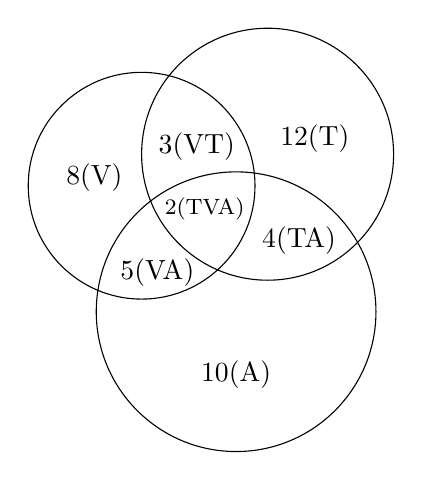
\begin{tikzpicture}[scale=.8]
				\def\radius{2cm}	
				\coordinate (ceni);
				\coordinate[xshift=.8*\radius, yshift=.2*\radius] (cenii);
				\coordinate[xshift=.6*\radius,yshift=-.8*\radius] (ceniii);
				\draw (ceni) circle (.9*\radius);
				\draw (cenii) circle (\radius);
				\draw (ceniii) circle (1.11*\radius);
				
				\node[xshift=-.3*\radius, yshift=.05*\radius] at (ceni) {$8$(V)};
				\node[xshift=.35*\radius, yshift=.25*\radius] at (ceni) {$3$(VT)};
				\node[xshift=.1*\radius, yshift=-.55*\radius] at (ceni) {$5$(VA)};
				\node[xshift=.4*\radius, yshift=-.15*\radius] at (ceni) {{\footnotesize $2$(TVA)}};
				\node[xshift=.2*\radius, yshift=-.55*\radius] at (cenii) {$4$(TA)};
				\node[xshift=1.1*\radius,yshift=.3*\radius] at (ceni) {$12$(T)};
				\node[yshift=-.4*\radius] at (ceniii) {$10$(A)};
			\end{tikzpicture}
		}
	}
\end{bt}

\begin{bt}%[0D1B3-3]
	Để thành lập đội tuyển học sinh giỏi khối $ 10 $, nhà trường tổ chức thi chọn các môn Toán, Văn, Anh trên tổng số $ 111 $ học sinh. Kết quả có: $ 70 $ học sinh giỏi Toán, $ 65 $ học sinh giỏi Văn, $ 62 $ học sinh giỏi Anh. Trong đó có $ 49 $ học sinh giỏi cả hai môn Văn và Toán, $ 32 $ học sinh giỏi cả hai môn Toán và Anh, $ 34 $ học sinh giỏi cả hai môn Văn và Anh. Xác định số học sinh giỏi cả ba môn Văn, Toán, Anh. Biết rằng có $ 6 $ học sinh không đạt yêu cầu cả ba môn.
	\loigiai{
		\immini
		{Có $ 111-6=105 $ học sinh thi đạt ít nhất $ 1 $ môn.\\
			Gọi $ A $ là số học sinh giỏi môn Toán và Tiếng Anh nhưng không giỏi Văn.\\
			Gọi $ B $ là số học sinh giỏi môn Toán và Văn nhưng không giỏi Tiếng Anh.\\
			Gọi $ C $ là số học sinh giỏi môn Văn và Tiếng Anh nhưng không giỏi Toán.\\
			Gọi $ D $ là số học sinh giỏi cả ba môn. Ta có hệ:\\
			$\begin{cases}
				B+D=49\\
				A+D=32\\
				C+D=34\\
				70+65+62-(A+B+C+2D)=105
			\end{cases}\\
			\Rightarrow 92=32-D+49-D+34-D+2D\\
			\Rightarrow D=23$.\\
			Vậy có $ 23 $ học sinh giỏi cả ba môn.
		}
		{
			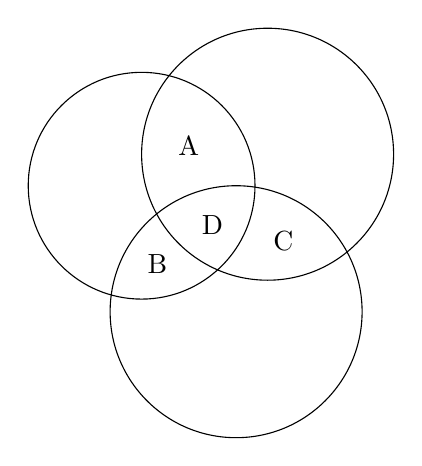
\begin{tikzpicture}[scale=.8]
				\def\radius{2cm}	
				\coordinate (ceni);
				\coordinate[xshift=.8*\radius, yshift=.2*\radius] (cenii);
				\coordinate[xshift=.6*\radius,yshift=-.8*\radius] (ceniii);
				\draw (ceni) circle (.9*\radius);
				\draw (cenii) circle (\radius);
				\draw (ceniii) circle (\radius);
				
				\node[xshift=.3*\radius, yshift=.25*\radius] at (ceni) {A};
				\node[xshift=.1*\radius, yshift=-.5*\radius] at (ceni) {B};
				\node[xshift=.45*\radius, yshift=-.25*\radius] at (ceni) {D};
				\node[xshift=.1*\radius, yshift=-.55*\radius] at (cenii) {C};
		\end{tikzpicture}}
	}
\end{bt}
